%
% Interface to Sector Logic
%

The track vector information from the NSW is combined with the results from the Big Wheel TGC (BW-TGC) by the new Sector Logic board located in USA-15.
The partitioning of the Trigger Sectors and granularities of the Regions-of-Interest (RoI) for the new Sector Logic board are the same as for the current \PhaseZero\ system. The same optical links and data format is used for signals from the BW-TGC, while new input optical links have been introduced to receive the NSW trigger information.

The BW-TGC, which covers the range of $1.0 < |\eta| < 2.4$, consists of three stations (TGC1, TGC2 and TGC3). The trigger algorithm extrapolates pivot-plane (TGC3) hits to the IP to construct roads following the infinite-momentum (straight) path for a track.
Deviations ($\Delta R$ and $\Delta\phi$) from this path of hits in the trigger planes are related to the momentum of the track.
Coincidence signals\footnote{The TGC1 station has three layers and the outer two stations (TGC2 and TGC3) each have two layers, resulting in a total of seven layers. A 3-out-of-4 coincidence is required for the doublet planes of TGC2 and TGC3, for both wires and strips; a 2-out-of-3 coincidence is required for the triplet (TGC1) wire planes; and 1-out-of-2 possible hits for the triplet strip planes.} are generated independently for $R$ and $\phi$.
The hit position information with granularity of RoIs and deviations ($R$ and $\Delta\phi$) is sent to the Sector Logic board.

The NSW information on the candidate track vectors, which are pointing to the IP within $\pm (7 - 15)$~mrad deviations\footnote{The value of this requirement is configurable and it will be optimized once better trigger simulation is available.}, are provided to the Sector Logic: the position ($R$ and $\Delta\phi$) and the deviation of the incidence angle at the NSW from a straight line to the IP ($\Delta\theta$).
In \PhaseOne, the final trigger decision is taken solely by merging the $R - \phi$ coincidence of signals from the BW-TGC and the NSW. In \PhaseTwo, the $\Delta\theta$ information will be combined with similar information from the BW chambers to improve the background rejection and sharpen the trigger threshold.
Since the NSW trigger system needs to be compatible with the \PhaseTwo requirements, the angle $\Delta\theta$ is required to be measured with an accuracy close to 1\,mrad even in \PhaseOne.


\subsubsection{NSW Trigger Data Format}
\label{ssec:specs-TriggerFormat}

The output data format of a track segment from the NSW trigger processor is shown in Table~\ref{tab:DataFormat}. One track segment is represented as 24~bits of data, which consist of 2~bits of segment-type information for each detector (\stgc and \MM), 5~bits for $\Delta\theta$, and 6~bits and 8~bits for $\phi$ and $R$ position information, respectively. Required resolutions (1~bit) are approximately 1~mrad ($\pm$15~mrad full scale) for $\Delta\theta$, 20~mrad for $\phi$ and 0.005 in pseudo-rapidity $\eta$.

The 2-bit segment-type information can provide an indication of the segment candidate quality, in addition to the detector. A value other than 00 indicates the segment was found by the corresponding detector. Up to a 3-level categorization can be encoded (01, 10 and 11), but the specific definitions are not yet established. 

Even though the sector logic is blind to the track segment origin (either \MM or \stgc) and quality, the segment-type bits should still be transmitted. They can be used to monitor the trigger operation, $e.g.$ to study the BW matches for each segment-type. The latency saved by omitting these four bits per candidate is small.


\begin{table}[h]
    \begin{center}
    \begin{tabular}{|c|c|c|c|c|c|c|}
    \hline
    Field:     & sTGC type & MM type & $\Delta\theta$ (mrad) & $\phi$ index &  $R$ index  &  spare  \\
    \hline
    Num of bits: &    2    &    2     &     5    &    6    &    8   &  1 \\
    \hline
    \end{tabular}
    \end{center}
    \caption{Data format of the output of the trigger processor sent to the Sector Logic. Format of a track vector candidate from the NSW (24-bits/track vector). The \stgc and \MM type information can encode the quality of the candidate.}
    \label{tab:DataFormat}
\end{table}


The data is transmitted from the \stgc and \MM trigger processors to the Sector Logic via optical fibres. The baseline is to send eight candidates per LHC bunch crossing (40~MHz) on two fibers, four candidates per stream, at 6.4\,Gb/s, 128~bit, using 8b/10b encoding. Figure\,\ref{fig:DataFormat} shows the format of the transmitted data. It is comprised of two IDLE codes for alignment purposes, three bytes of data for up to four track segments, the NSW Sector ID (4~bits) and a BCID number (12\,bits). Each 2-byte word is transferred after 8b/10b encoding at 320\,MHz.


\begin{figure}[h]
    \begin{center}
        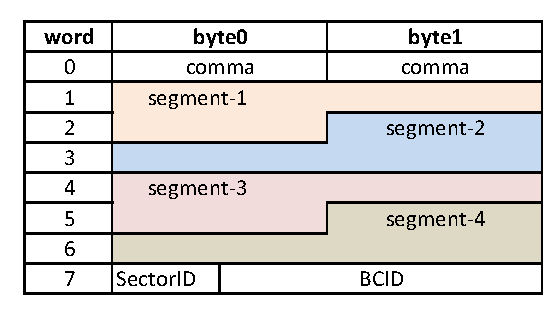
\includegraphics[width=0.55\textwidth]{specs/NSWtoSectorLogicFmt.pdf}
        \caption{Data format from the NSW trigger processor to the Sector Logic. The data is transmitted with 8b/10b encoding in one bunch crossing (16\,bytes at 6.4\,Gbps). The 24-bit segment format is shown in Table~\ref{tab:DataFormat}. The comma character is an idle code for alignment purposes in the 8b/10b encoding.
        The NSW Sector ID is 4~bits and the BCID is 12~bits.}
        \label{fig:DataFormat}
    \end{center}
\end{figure}

%The model of the trigger in the Athena simulation of both the sTGC and the MM trigger is incomplete. There is also a need to simulate correlated backgrounds. As a result, the probability to find track segments as a function of the radius is not known. The main quantities of interest are the probability of finding more than four \stgc or \MM candidates, as well as more than eight total candidates when duplicates are removed.

\paragraph{Data overflow}Information about data overflow is planned to be added. An overflow bit would be set if, for a BCID, more than the maximum number of transmittable candidates is found, and thus incomplete information is sent. One possibility is to use the reserved bit of the last track candidate word sent to the Sector Logic. This option requires no additional bits. 

If the simulation shows that eight candidates are insufficient, the following possibilities, although highly undesirable, could be considered to enable transmitting up to 12 candidates:
\begin{itemize}
\item Increase from two to three fibres. This option would exceed the number of serializers available with the intended Kintex FPGA and increase the complexity of the Sector Logic.
Recently, however, it was found that the Sector Logic boards may in fact be able to handle up to 10 links from the NSW, instead of six, as initially thought. This means that a third fiber might be available in case of need. More studies would be necessary to explore the eventual use of this possibility, which is not our baseline.
\item Transmission at 9.6 Gb/s, however the Kintex GTX cannot operate at this rate (higher or lower is OK). Note that this does not require any change at the Trigger Processor end.
\item Transmission at 8 Gb/s which would be sufficient to provide 10 candidates.
\end{itemize}


\subsubsection{Combination of sTGC and MM trigger data}
\label{ssec:specs-combination}
% Combination of sTGC and MM trigger data
%

The \MM and \stgc trigger processors compute track vectors independently. The \stgc trigger produces a maximum of four candidates per sector, driven by its hardware design.
The \MM trigger has no such limitation and can theoretically find more candidates if they are present. 

%Both \stgc and \MM trigger processors belonging to a NSW \sector will be in the same ATCA board~\cite{hardware-LAr-Carrier,hardware-SRS-Carrier}, although their information is processed by separate algorithms (see Section~\ref{sec:algorithms}) in separate FPGAs. 

The \stgc and \MM trigger information from one NSW \sector will be processed in the same Trigger Processor ATCA board~\cite{hardware-SRS-Carrier,hardware-LAr-Carrier}. The two algorithms (see Section~\ref{sec:algorithms}) will run in separate FPGAs, connected by several high-speed, low latency differential LVDS pairs.
Depending on the hardware platform chosen the two FPGAs will be located in one (SRS option~\cite{hardware-SRS-Mezz}) or two  (LAr option~\cite{hardware-LAr-OTC}) mezzanine cards. 
A NSW trigger processor ATCA board serves one NSW octant, i.e. two NSW sectors, and therefore
contains two or four mezzanine cards (depending on the hardware platform).
A comparison of the two platforms is provided in Section~\ref{sec:hardware-platforms}.

%A NSW trigger processor ATCA board (corresponding to two NSW sectors) contains two or four mezzanine cards (depending on the hardware platform ultimately chosen) and therefore serves a NSW octant

Given that the \MM trigger system is expected to be faster than the \stgc one, the \MM trigger results will be sent 
to the \stgc FPGA for the stream merging stage. This procedure eliminates the impact on the latency due to the data transfer. The merging algorithm, which includes duplicate removal, is expected to take up to 50 ns, 
increasing the overall NSW latency budget to 43 BCs. The actual algorithm implementation is however needed for a full evaluation of its impact on the latency.

In order to implement the merging algorithm, the fast connectivity between the \MM and \stgc FPGAs is imperative.
In the current design, the SRS option offers 64 LVDS high-speed connections between the FPGAs, which would fully satisfy the bandwidth requirements, while the LAr option only offers eight.
Studies are on-going to determine by how much this number could be increased.

The trigger stream merging will limit the number of NSW track vector candidates to eight (subject to simulation results, see Section~\ref{ssec:specs-TriggerFormat}). Possible selection criteria of track vectors are:
\begin{itemize}
	\item Remove duplicates, where a duplicate is a candidate with the same $R$ and $\phi$, and similar $\Delta\theta$. The conditions for a $\Delta\theta$ match still need to be evaluated taking into account the intrinsic resolutions and the relative alignment of the two detectors.
	\item Select according to a `quality' flag defined by the trigger algorithm. For example, if the vector was produced from only one of the two four-layer modules of the \stgc because the track passed through a support in the second module, its resolution is degraded and the vector would have a lower quality.
\end{itemize}

Although both \stgc and \MM trigger modules are in the same ATCA board with high bandwidth connectivity, an algorithm that would merge hits and then find vectors has been disfavored at this time due to the additional latency requirements and increased complexity.

%Handling the details of the detector differences at the hit level would require more processing time than is available in the \PhaseOne latency budget.
%Any improvement of the vectors' accuracy from such an algorithm may not be needed, at least for \PhaseOne, and the added complexity may not be justified.


\subsubsection{Matching to Sector Logic Boards}
\label{ssec:specs-sl-boards}

Figure~\ref{fig:L1MuEC-TriggerSector} shows the projection of the NSW sectors into the BW-TGC pivot plane which is divided into two regions, end-cap ($|\eta|<1.9$) and forward ($|\eta|>1.9$). The end-cap region is divided into 48 trigger sectors in $\phi$, while the forward region is divided into 24 trigger sectors. A trigger sector, represented in the figure by the green lines, is a logical unit that is treated independently in the trigger\footnote{Remember that the TGC has 12 detector sectors. Thus, each TGC detector sector comprises four end-cap trigger sectors and two forward trigger sectors.}.

The thick red lines in Figure~\ref{fig:L1MuEC-TriggerSector} show the projective boundaries of the NSW detector, which covers $1.3<|\eta|<2.4$ and whose structure has octant symmetry. 
Each octant has a large NSW sector and a small NSW sector\footnote{Note that in the NSW the detector and trigger sectors are coincidental, unlike in the case of the BW-TGC.}, corresponding to 16 NSW Trigger Sectors per endcap. 
The boundaries of the NSW sectors (indicated by the red lines) do not coincide with the segmentation of the BW-TGC trigger sectors. Each large NSW sector geometrically covers six BW-TGC Trigger Sectors, while each small NSW sectors covers seven (notice the very thin overlap regions in the NSW small sector case). 

To take into account deformations in the endcap magnetic field, multiple scattering and misalignments, one NSW sector also needs to deliver information to the BW-TGC sectors adjacent to the geometrically overlapping ones.
This means that the information from a large NSW sector has to be corroborated with that of six \endcap trigger sectors and four forward trigger sectors.
Similarly, information from a small NSW sector has to be combined with four \endcap trigger sectors and three forward trigger sectors.

The granularity of the Regions-of-Interest is indicated by the thin red lines. The sizes of the RoIs are approximately 0.025$\times$0.030 in \etaphi. There are 560 (366) RoIs corresponding to each large (small) NSW sector.
%{\bf (I counted a slightly different number: large - (12+14)*4*4 + 16*4*2 = 416 + 128 = 544; (12+14)*5*2 + 16*6 = 260 + 96 = 356).}

\begin{figure}[htb]
  \centering
  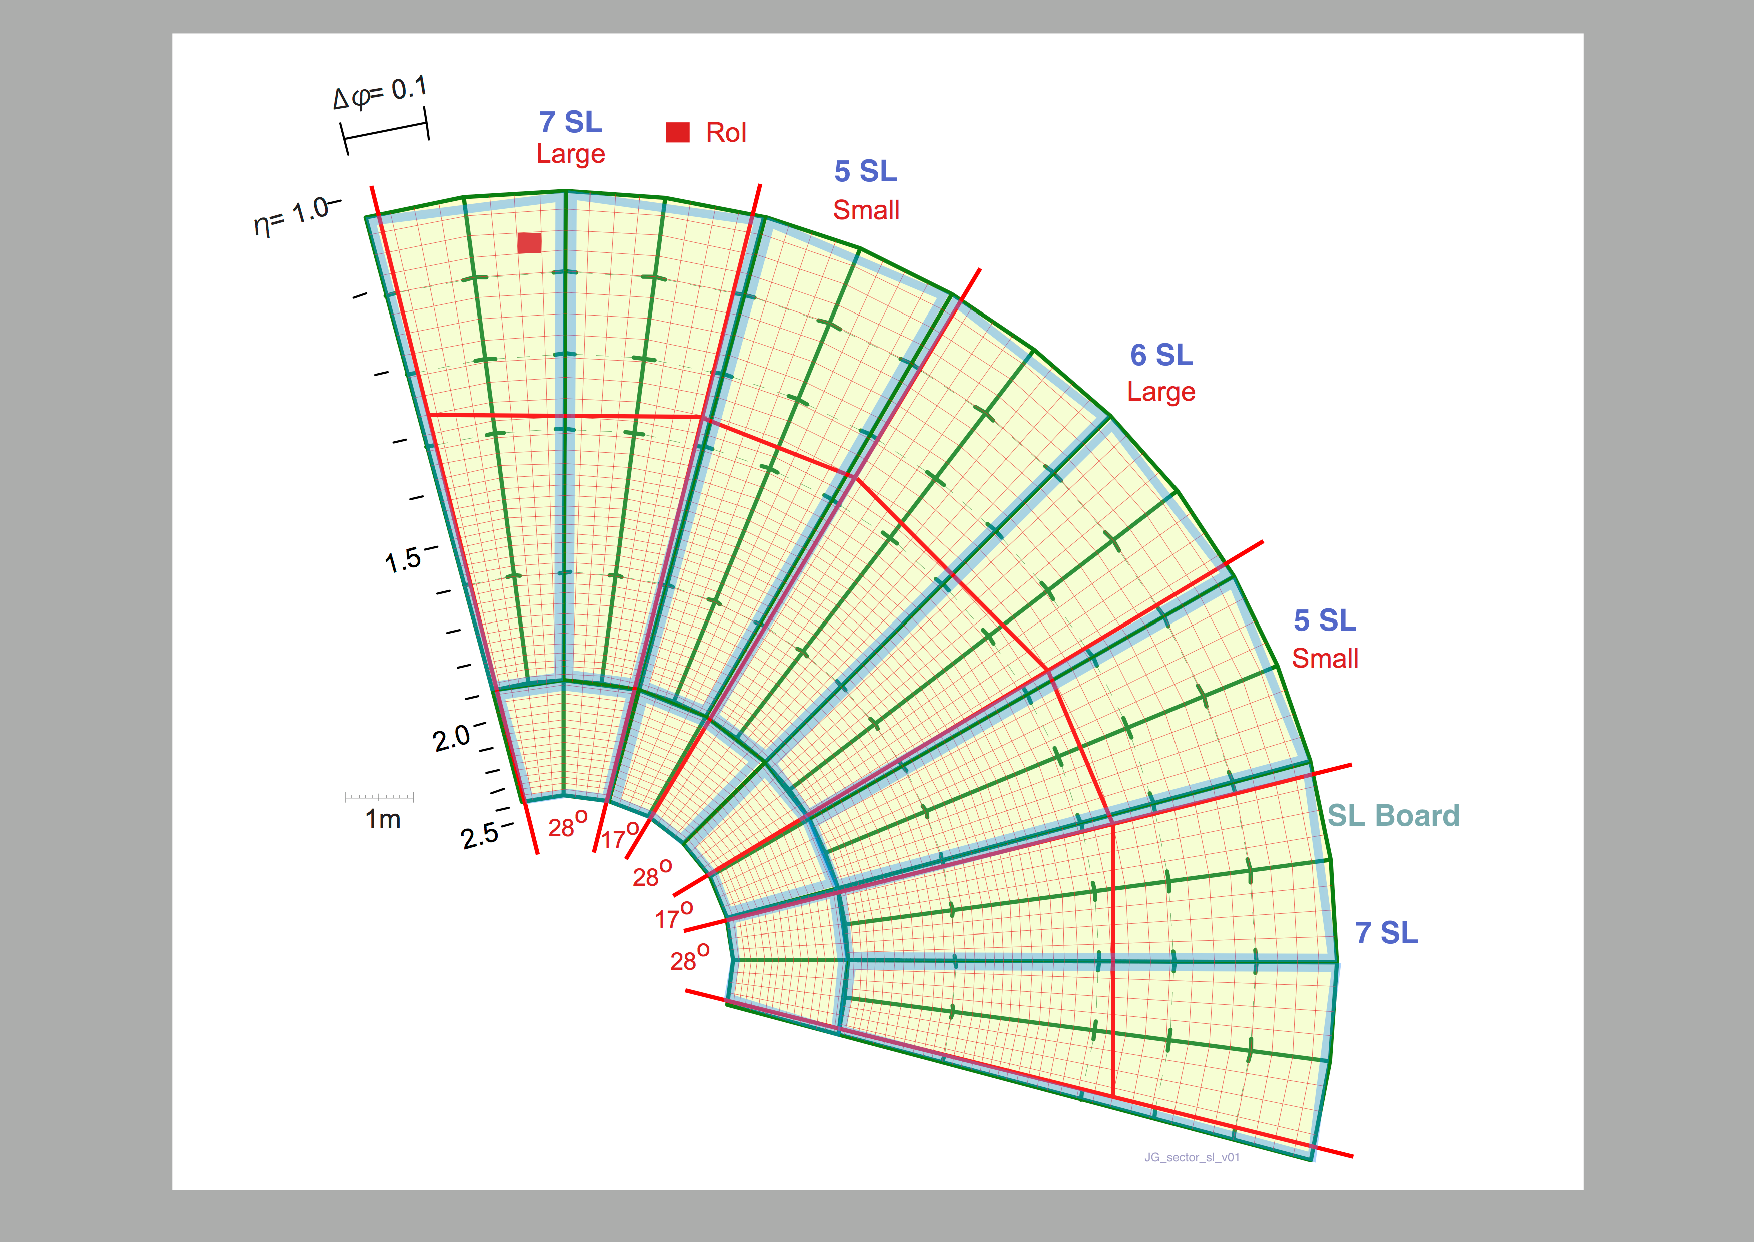
\includegraphics[trim=4cm 1.0cm 4.7cm 1.0cm, clip=true, width=0.8\textwidth]{specs/JG_sector_sl_v01.pdf}
  %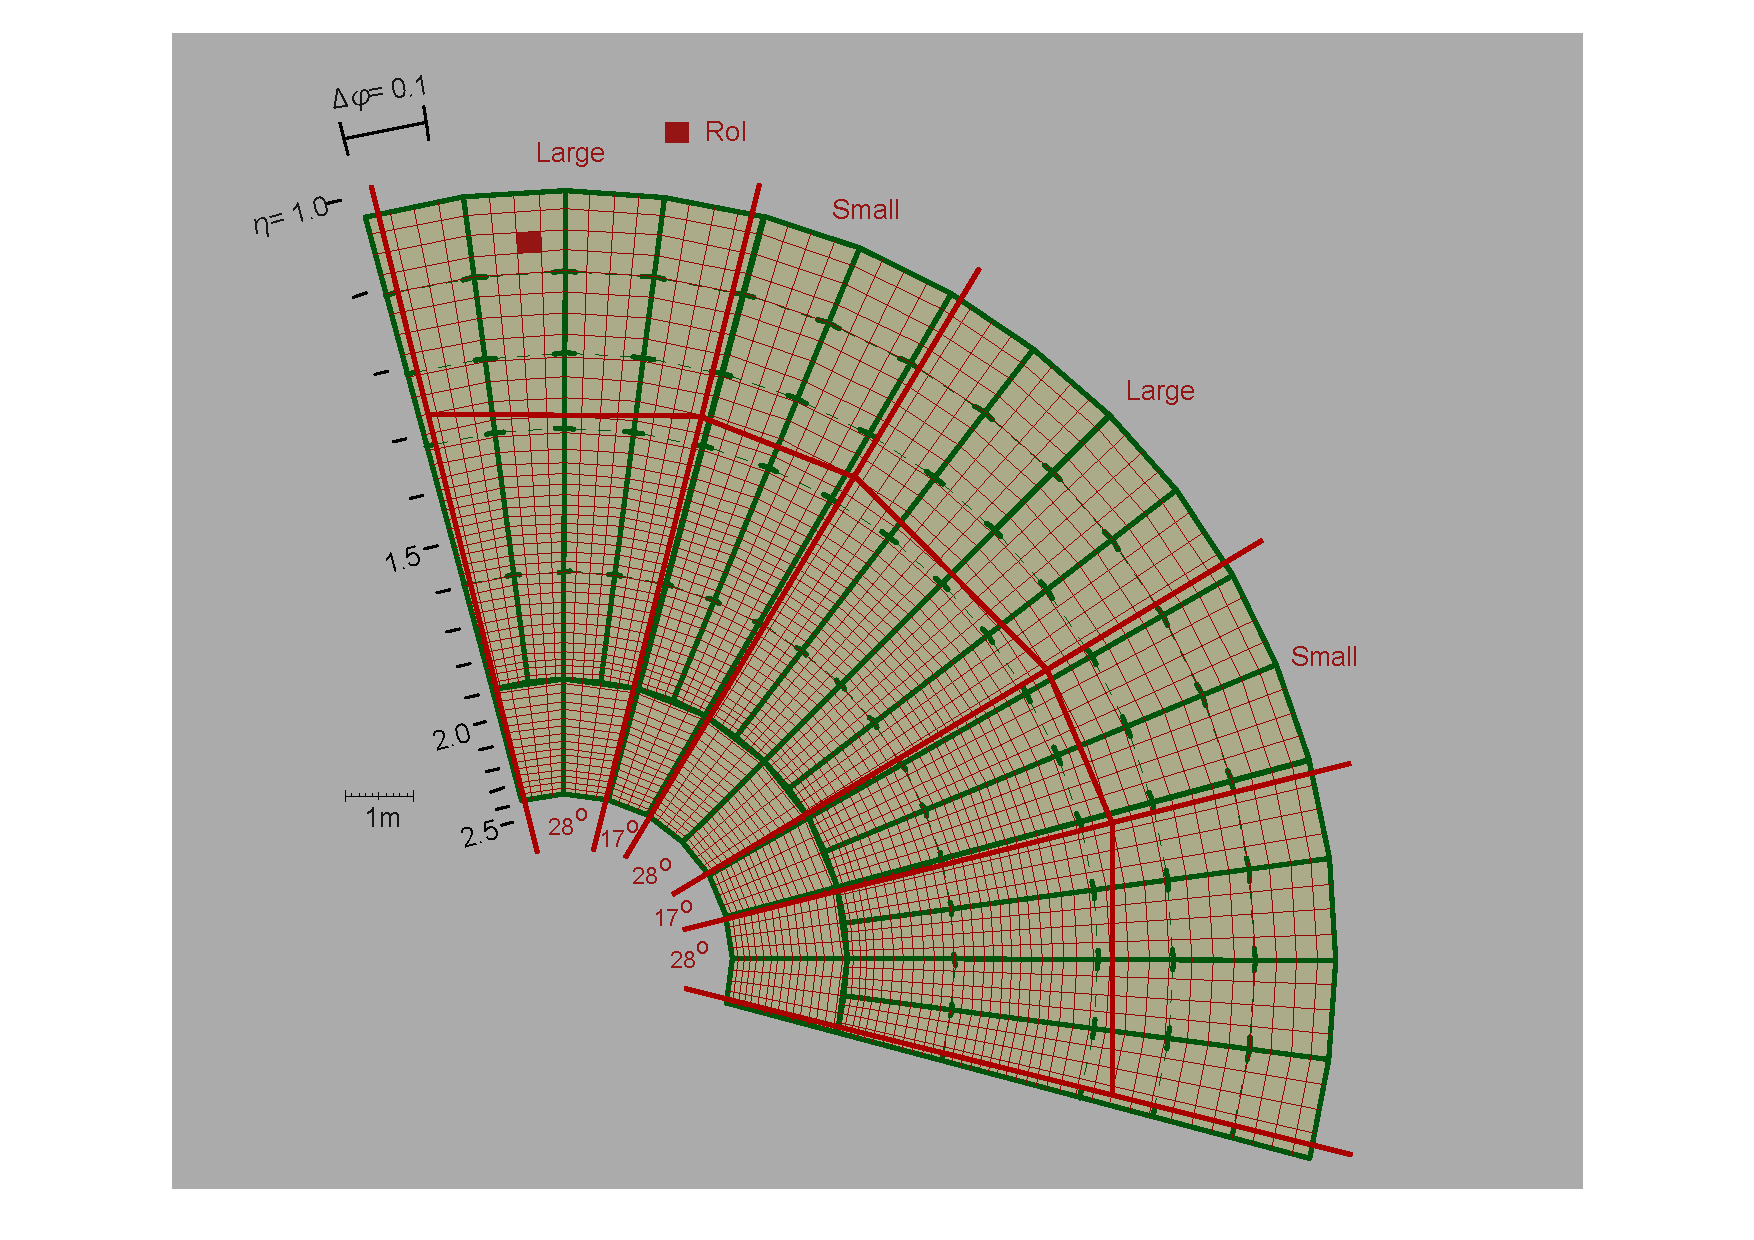
\includegraphics[trim=4cm 1.0cm 6.5cm 1.0cm, clip=true, width=0.7\textwidth]{specs/sector.pdf}  
 \caption{Trigger Sector segmentation (green lines) and projection of the NSW sectors (thick red lines) into the pivot plane (TGC3). The blue shapes represent the coverage of a SL board. The number of SL boards covered by each NSW sector is indicated in blue.}
  \label{fig:L1MuEC-TriggerSector}
\end{figure}

There are two types of Sector Logic boards, the ``\Endcap Sector Logic'' board and the ``Forward Sector Logic'' board. A single Sector Logic board serves two adjacent trigger sectors, therefore 24 Endcap and 12 Forward Sector Logic boards per side are required.
Figure~\ref{fig:L1MuEC-TriggerSector} shows the mapping of the SL boards (in blue) to the trigger sectors. The trigger information from each NSW trigger sector is fanned-out and delivered to the corresponding SL boards. There will be five to seven replicas required from each NSW sector because a single SL board serves two trigger sectors. 
This maximum number of signal fan-out is needed for the NSW large sector.



%Figure~\ref{fig:L1MuEC-FanoutScheme} shows the signal distribution scheme from the NSW to the Sector Logic
%boards. Vector data of track segments, which are found in sTGCs and MicroMegas separately, are merged by the NSW trigger electronics. Combined track information is fanned-out and delivered to corresponding Sector Logic boards.

Several replication possibilities are currently being considered:
\begin{description}
    \item [1:7 fan-out with active fan-outs:] slightly higher latency due to optical-electrical-optical conversion and additional fiber length
    \item [1:7 fan-out with passive optical splitter:] rejected since signal loss is too high
    \item [2$\times$(1:4) passive optical splitter:] perhaps possible, depending if the transmitter optical power is sufficient. Would need to be checked and/or tested.
    \item [4$\times$(1:2) passive optical splitter:] OK, but only if the trigger processor has enough outputs.  Requires eight output optical links.
    \item [7 fibers directly from TP:] OK, but only if the trigger processor has enough outputs. Requires 14 output optical links.
\end{description}

At this point, both platform options should be able to provide 14 optical output links for this purpose. Pending a deeper evaluation, the baseline is that the TP will provide the seven streams (2 x 7 fibers) directly to the SL, without the need for a fan-out, as shown in Figure~\ref{fig:Interface-TP-SL}.
Note however that neither the opto-electronics for additional links nor the fan-outs have been included in the NSW costing.

\begin{figure}[htb]
  \centering
  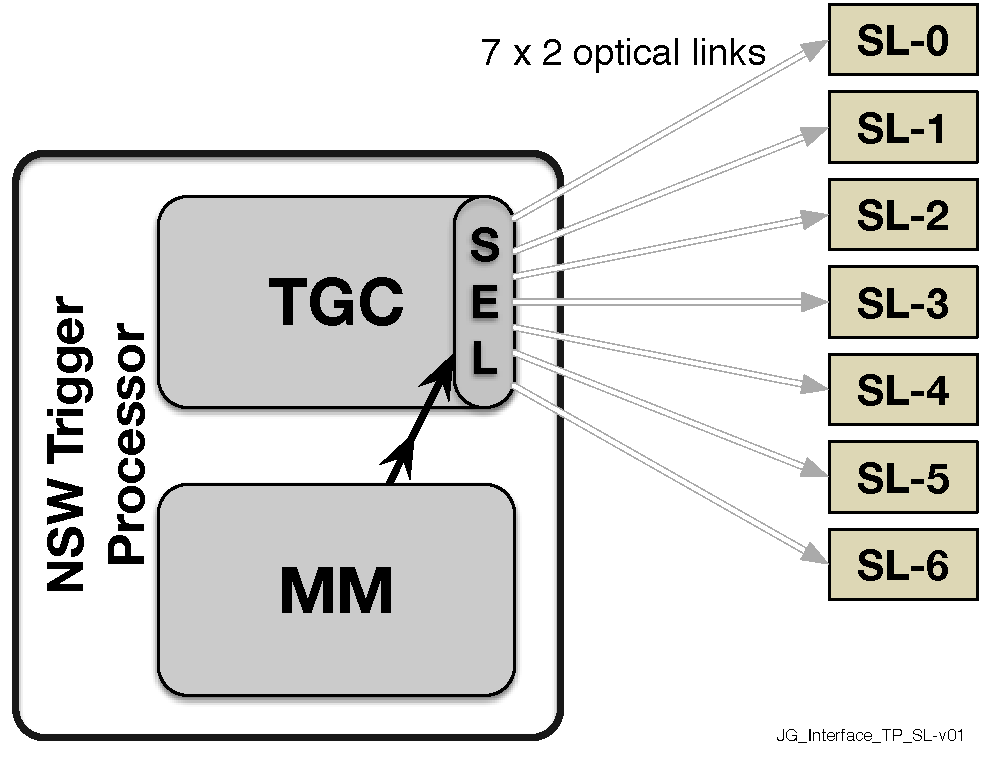
\includegraphics[width=0.4\textwidth]{specs/JG_Interface_TP_SL-v01}
 \caption{Interface between the NSW trigger electronics and the Sector Logic.
 One NSW trigger sector will connect to up to seven SL boards via optical links.}
  \label{fig:Interface-TP-SL}
\end{figure}


It has also been proposed that splitting the fibers, at the NSW Trigger Processor, as belonging to different $\phi$ regions within a sector might reduce the need to fan-out the output, without compromising the maximum number of candidates transmitted. This would however introduce undesirable hard boundaries into the SL. A third fiber from inner regions of the large sectors might also be used. More studies would be needed to explore these possibilities.


%{\bf Stuff below here is to be removed}
%
%\begin{enumerate}
%  \setlength{\itemsep}{1pt}
%  \setlength{\parskip}{0pt}
%  \setlength{\parsep}{0pt}
%        \item   Send trigger segments to Sector Logic
%        \begin{enumerate}
%        \item   Steps required
%        \begin{enumerate}
%        \item   Construct $\Delta\theta$, and ROI locations of each candidate in appropriate format (as given in Figure~\ref{fig:DataFormat})
%        \item   Synchronize to BC domain and output on required BCID
%        \item   Serialize for transmission to Sector Logic using Xilinx GTX core
%        \begin{enumerate}
%        \item   Encode with 8b/10b (VHDL from FELIX)
%        \end{enumerate}
%        \end{enumerate}
%        \item   Failure modes and recovery
%        \begin{enumerate}
%        \item   Too many segments for transmission – truncate list to maximum allowed; send exception message.
%        \end{enumerate}
%        \end{enumerate}
%\end{enumerate}
